\documentclass[tikz,border=6pt]{standalone}
% Shared visual language for the original benchmark atlas.
\usepackage[T1]{fontenc}
\usepackage{lmodern}
\usepackage{amsmath,amssymb}
\usetikzlibrary{arrows.meta,calc,positioning,shapes.geometric,patterns,decorations.pathmorphing,backgrounds,fit}
\definecolor{ink}{HTML}{173948}
\definecolor{flow}{HTML}{167D9A}
\definecolor{control}{HTML}{A65217}
\definecolor{measure}{HTML}{70518A}
\definecolor{pale}{HTML}{EAF2F5}
\definecolor{muted}{HTML}{526571}
\definecolor{utility}{HTML}{2E8665}
\tikzset{
  every node/.style={font=\sffamily\small,text=ink},
  equipment/.style={draw=ink,line width=1pt,fill=pale,rounded corners=2pt},
  process/.style={draw=flow,line width=1.2pt,-{Latex[length=2.5mm]}},
  signal/.style={draw=control,line width=.8pt,dashed,-{Latex[length=2mm]}},
  util/.style={draw=utility,line width=1pt,-{Latex[length=2.2mm]}},
  dimension/.style={draw=muted,line width=.6pt,{Latex[length=1.7mm]}-{Latex[length=1.7mm]}},
  labelbox/.style={fill=white,inner sep=2pt,font=\sffamily\footnotesize,align=center},
  annotation/.style={font=\sffamily\footnotesize,text=muted,align=left},
  panel/.style={draw=ink!20,fill=ink!2,rounded corners=3pt,inner sep=6pt},
  instrument/.style={circle,draw=measure,fill=white,line width=.8pt,minimum size=8mm,inner sep=1pt,font=\sffamily\scriptsize,align=center},
  port/.style={circle,fill=flow,inner sep=1.6pt},
  box/.style={equipment,minimum width=3cm,minimum height=1cm,align=center},
}
\newcommand{\atlasheader}[3]{%
  \node[anchor=north west,font=\sffamily\bfseries\LARGE] at (0,0) {#1};%
  \node[anchor=north west,font=\sffamily\small,text=muted] at (0,-.75) {Paper section #2: \textit{#3}};%
  \draw[ink!25,line width=.7pt] (0,-1.25)--(26,-1.25);%
}
\newcommand{\atlasfooter}[1]{%
  \draw[ink!25,line width=.5pt] (0,-15.8)--(26,-15.8);%
  \node[anchor=north west,annotation,text width=25.8cm] at (0,-16) {#1\\Original explanatory drawing. Source: Kroll \& Schulte (2014), DOI: 10.1016/j.asoc.2014.08.034. Model variants are identified in the accompanying case sheet.};%
}

% Wind-turbine-only finish; keep the remainder of the benchmark atlas unchanged.
% TikZ.net methods: material shading and directional flow layers:
% https://tikz.net/fluid_dynamics_laminar/
% TikZ.net methods: named model nodes and coordinated input/output routes:
% https://tikz.net/mechanics/
% Component organization cross-check (shaft -> gearbox -> generator):
% https://www.mdpi.com/1996-1944/15/3/1232 (nacelle schematic; not a construction detail)
% Real-world material cues (matte pale blades, coated steel towers and nacelle shells):
% https://www.energy.gov/sites/prod/files/2017/08/f35/EA-2045_Draft%20Environmental%20Assessment.pdf
% https://docs.nrel.gov/docs/fy25osti/87970.pdf
% Exact tints, highlights, cast shadows, and equipment internals are illustrative,
% NOT a material specification or a photorealistic model of a particular turbine.
\usetikzlibrary{shadows}
\definecolor{ink}{HTML}{263A45}
\definecolor{flow}{HTML}{2885AE}
\definecolor{utility}{HTML}{168373}
\definecolor{control}{HTML}{BD682F}
\definecolor{muted}{HTML}{586B74}
\definecolor{pale}{HTML}{F3F5F2}
\definecolor{steelrim}{HTML}{485E66}
\definecolor{steelshade}{HTML}{93A9B4}
\definecolor{steelmid}{HTML}{CFDFE1}
\definecolor{steelhi}{HTML}{FFFEF8}
\definecolor{steelblue}{HTML}{6E8798}
\definecolor{compositeLit}{HTML}{FEFCF3}
\definecolor{compositeMid}{HTML}{E9E7DC}
\definecolor{compositeShade}{HTML}{A4B9BF}
\definecolor{towerLit}{HTML}{FBF9F0}
\definecolor{towerMid}{HTML}{D8DBD6}
\definecolor{towerShade}{HTML}{8E9FA8}
\definecolor{nacelleShade}{HTML}{9FB2BB}
\definecolor{metalDark}{HTML}{344853}
\definecolor{metalSilver}{HTML}{C3D2D9}
\definecolor{bronze}{HTML}{B38358}
\definecolor{bronzeDark}{HTML}{795A47}
\definecolor{ground}{HTML}{CEC5B6}
\definecolor{skyWash}{HTML}{ECF6FA}
\definecolor{warmLight}{HTML}{FFFFF2}
\definecolor{rotorTint}{HTML}{E7F1F5}
\definecolor{shaftTint}{HTML}{F1ECE4}
\definecolor{generatorTint}{HTML}{E6EDF0}
\definecolor{aeroTint}{HTML}{E6F3EC}
\definecolor{pitchTint}{HTML}{FAEFE5}

\tikzset{
  every node/.style={font=\sffamily\small,text=ink},
  equipment/.style={draw=steelrim,line width=1.0pt,fill=pale,rounded corners=2pt},
  process/.style={draw=flow,line width=1.25pt,line cap=round,-{Triangle[length=2.4mm,width=1.7mm]}},
  signal/.style={draw=control,line width=.9pt,dash pattern=on 3.5pt off 2.3pt,line cap=round,-{Triangle[length=2.1mm,width=1.5mm]}},
  util/.style={draw=utility,line width=1.2pt,line cap=round,-{Triangle[length=2.3mm,width=1.7mm]}},
  dimension/.style={draw=muted,line width=.85pt,{Stealth[length=1.9mm,width=1.5mm]}-{Stealth[length=1.9mm,width=1.5mm]}},
  labelbox/.style={fill=white,inner xsep=3pt,inner ysep=2pt,font=\sffamily\footnotesize,align=center},
  annotation/.style={font=\sffamily\footnotesize,text=muted,align=left},
  panel/.style={draw=ink!18,fill=ink!2,rounded corners=3pt,inner sep=6pt},
  box/.style={equipment,minimum width=3cm,minimum height=1cm,align=center,
    drop shadow={opacity=.10,shadow xshift=1pt,shadow yshift=-1pt}},
}

\begin{document}
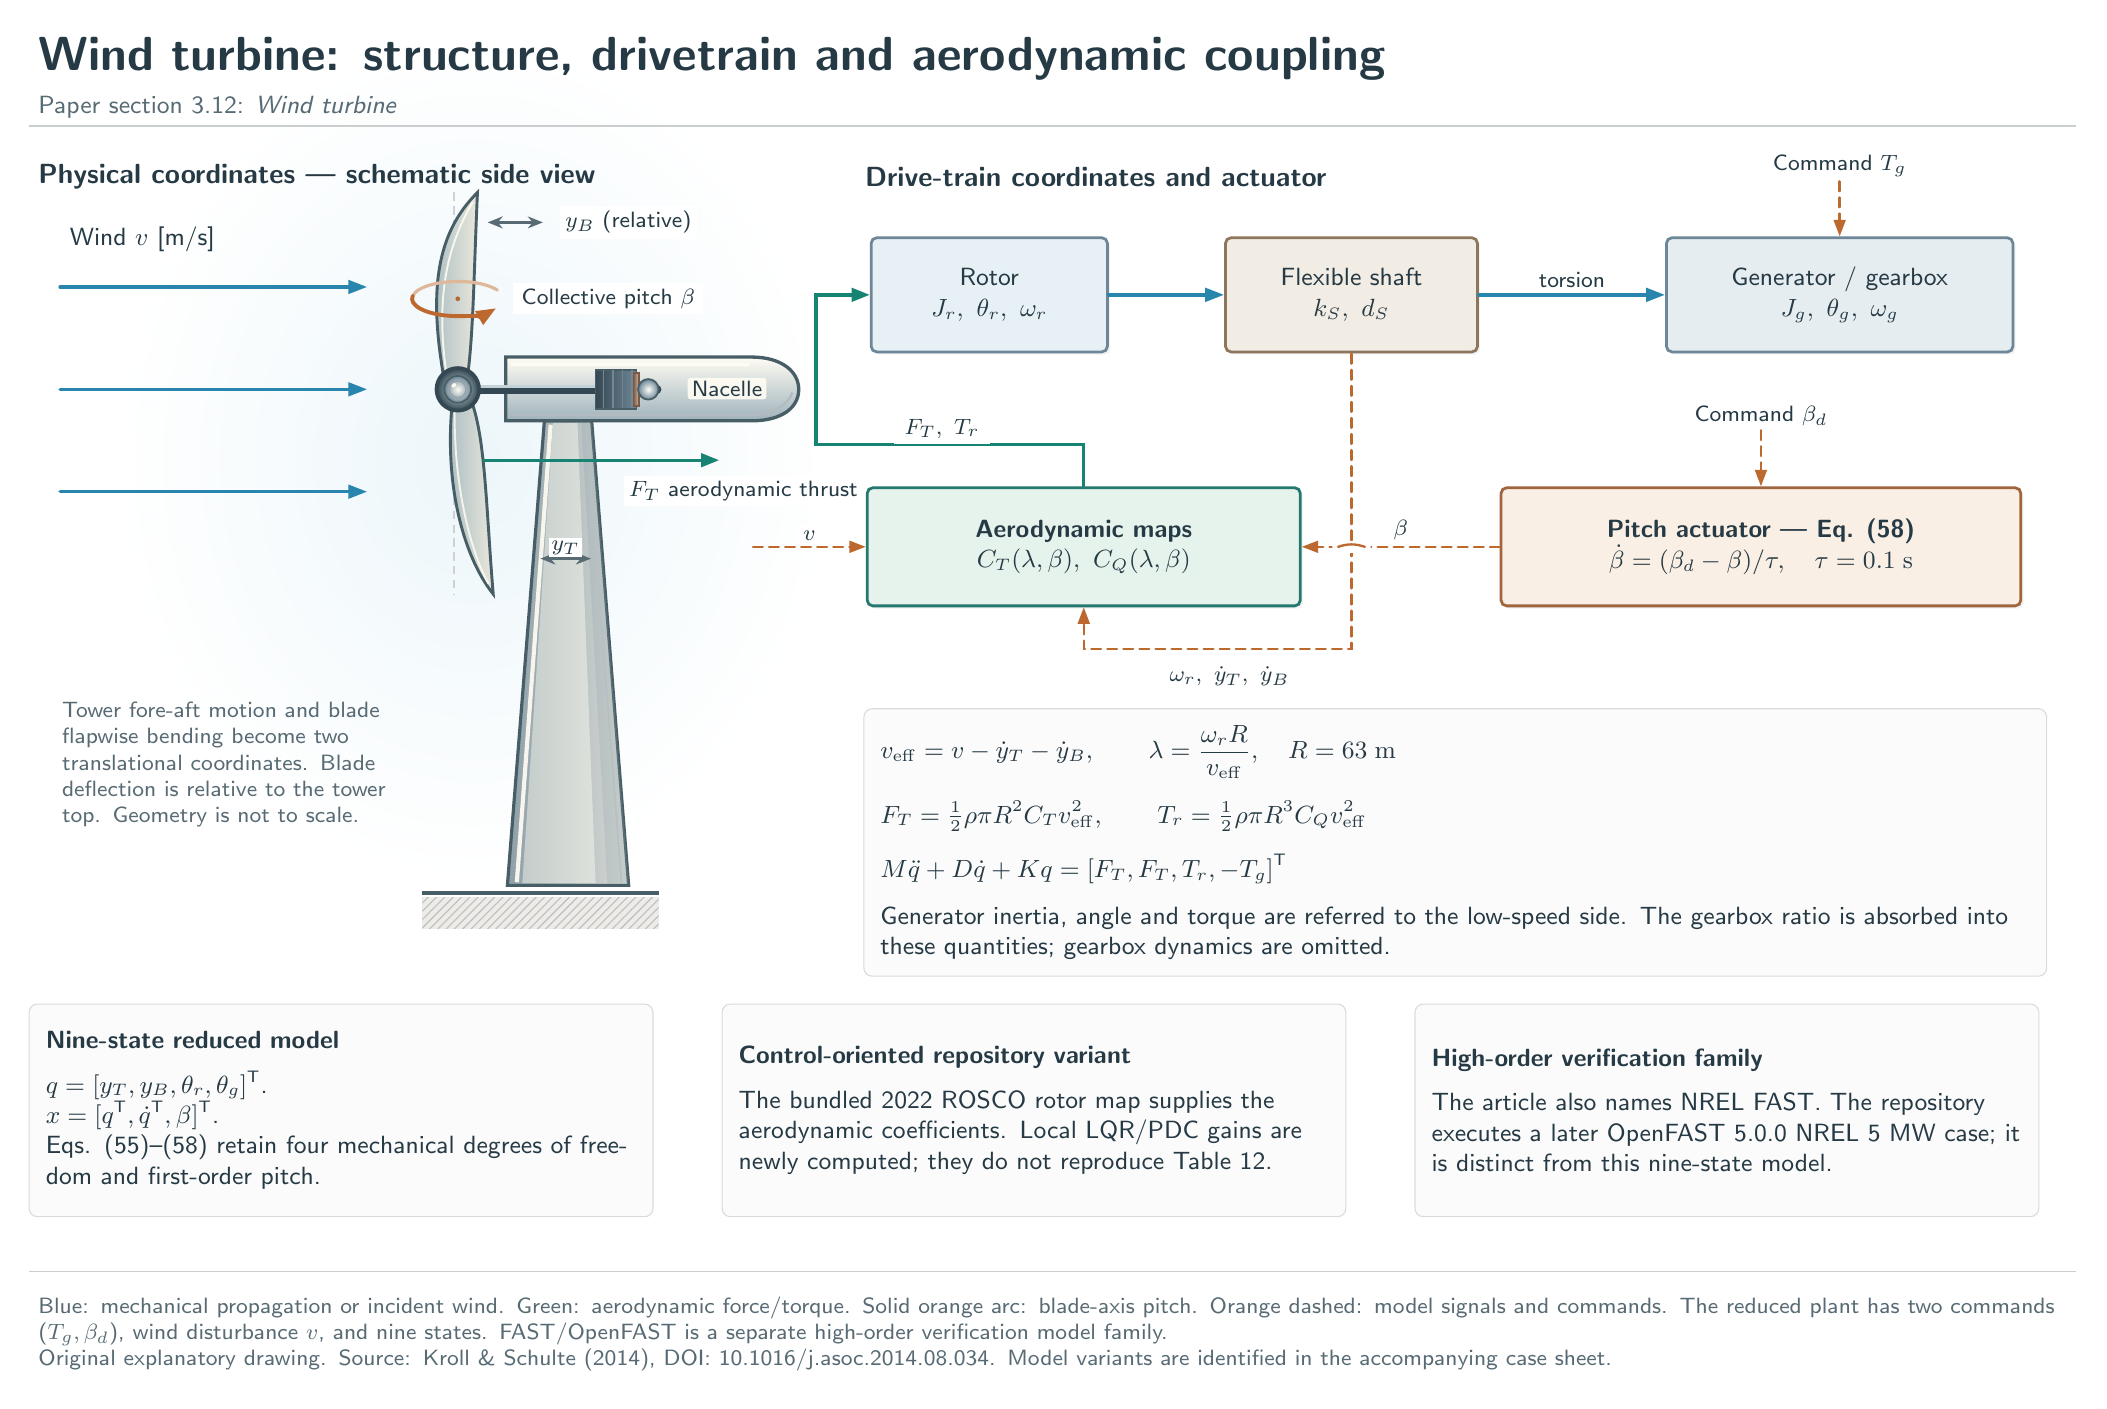
\begin{tikzpicture}[x=1cm,y=1cm]
% A pale ambient field belongs BEHIND all labels and lines, never above them.
\shade[inner color=skyWash,outer color=white] (5.65,-5.5) ellipse (4.55cm and 5.35cm);
\atlasheader{Wind turbine: structure, drivetrain and aerodynamic coupling}{3.12}{Wind turbine}
\node[anchor=west,font=\sffamily\bfseries] at (0,-1.9) {Physical coordinates --- schematic side view};
% Straight-sided, vertical tapered tower: both edges are linear, not curved.
% The tower centreline x=6.85 is vertical; cross-section widens toward foundation.
\draw[ink!28,densely dashed,line width=.7pt] (6.85,-10.9)--(6.85,-5.05);
% Painted-steel tapered tower: warm sunlit face / cool blue-gray shadow.
% Real wind-turbine towers are predominantly light gray/white, not polished chrome.
\shade[draw=steelrim,line width=1.15pt,
       left color=towerShade,middle color=towerLit,right color=towerMid]
 (6.55,-5.0)--(7.15,-5.0)--(7.62,-10.9)--(6.08,-10.9)--cycle;
% Lit painted face occupies a broad zone, not just a hairline highlight;
% softly darker starboard side keeps the shell cylindrical at diagram scale.
\path[fill=warmLight,opacity=.44]
 (6.66,-5.025)--(6.97,-5.025)--(7.20,-10.87)--(6.27,-10.87)--cycle;
\path[fill=towerShade,opacity=.23]
 (7.02,-5.025)--(7.15,-5.025)--(7.62,-10.88)--(7.35,-10.88)--cycle;
\draw[towerLit,line width=1.5pt,opacity=.96] (6.63,-5.05)--(6.20,-10.86);
\draw[steelrim!40,line width=.55pt] (7.08,-5.05)--(7.53,-10.87);
% Neutral foundation is distinct from the painted tower.
\fill[ground!32] (5,-11.05) rectangle (8,-11.45);
\fill[pattern=north east lines,pattern color=ink!32] (5,-11.05) rectangle (8,-11.45);
\draw[steelrim,line width=1.5pt] (5,-11)--(8,-11);
% Enclosed nacelle / illustrative machine internals, not vendor-specific hardware.
% Nacelle shell: warm pearl composite top, cool shaded underside, darker lip.
% Geometry is unchanged, only the illuminated surface treatment differs.
\shade[draw=steelrim,line width=1.2pt,
       top color=compositeLit,middle color=compositeMid,bottom color=nacelleShade]
 (6.06,-4.19)--(9.18,-4.19)
 ..controls (9.57,-4.19) and (9.78,-4.38)..(9.78,-4.60)
 ..controls (9.78,-4.83) and (9.57,-5.00)..(9.18,-5.00)
 --(6.06,-5.00)--cycle;
% Light catching its upper edge and form-following shadow under the rounded cap.
\draw[compositeLit,line width=1.0pt,opacity=.96] (6.13,-4.285)--(9.15,-4.285);
\draw[steelrim!42,line width=.8pt] (6.13,-4.925)--(9.15,-4.925)
 ..controls(9.43,-4.925)and(9.65,-4.80)..(9.70,-4.64);
% The rotor shaft passes continuously into a compact stylized drivetrain.
% Steel drivetrain: raised edge, recessed graphite shaft and copper-tone hub collar.
\draw[metalDark,line width=3.2pt,line cap=round] (5.35,-4.6)--(7.98,-4.6);
\draw[metalSilver,line width=1.10pt,line cap=round] (5.35,-4.562)--(7.98,-4.562);
% Compact gearbox housing: brushed blue-gray sides with restrained copper collar.
\shade[draw=steelrim,line width=.65pt,left color=metalDark,
       middle color=metalSilver,right color=steelblue]
 (7.20,-4.85) rectangle (7.72,-4.35);
\foreach \xx in {7.30,7.42,7.54,7.66}{
  \draw[steelrim!75,line width=.55pt](\xx,-4.84)--(\xx,-4.36);
}
\shade[draw=bronzeDark,line width=.55pt,left color=bronzeDark,right color=bronze!55!white]
 (7.68,-4.81) rectangle (7.75,-4.39);
\shade[draw=steelrim,line width=.65pt,inner color=steelhi,outer color=steelblue]
 (7.87,-4.60) circle (.13);
\node[font=\sffamily\footnotesize,fill=compositeLit,fill opacity=.92,
      text opacity=1,inner xsep=1.5pt,inner ysep=1.1pt,rounded corners=1pt]
 at (8.87,-4.59) {Nacelle};
% Fiberglass-composite airfoils: pale matte faces, shaded far edges, not metal.
\draw[ink!23,densely dashed,line width=.7pt] (5.4,-2.1)--(5.4,-7.2);
\shade[draw=steelrim,line width=1.05pt,
       left color=compositeShade,middle color=compositeLit,right color=compositeMid]
 (5.3,-4.6)..controls(5.05,-3.3)and(5.2,-2.6)..(5.7,-2.1)
 ..controls(5.65,-3.2)and(5.65,-4)..(5.55,-4.6)--cycle;
\draw[compositeLit,line width=.70pt,opacity=.88]
 (5.325,-4.53)..controls(5.15,-3.45)and(5.31,-2.79)..(5.64,-2.22);
\shade[draw=steelrim,line width=1.05pt,
       left color=compositeShade,middle color=compositeLit,right color=compositeMid]
 (5.4,-4.6)..controls(5.25,-5.7)and(5.5,-6.7)..(5.9,-7.2)
 ..controls(5.8,-6)and(5.8,-5)..(5.55,-4.6)--cycle;
\draw[compositeLit,line width=.70pt,opacity=.84]
 (5.415,-4.67)..controls(5.37,-5.78)and(5.62,-6.68)..(5.84,-7.07);
% Metallic rotor hub reads separately from pale composite blades.
\shade[draw=metalDark,line width=1.35pt,outer color=metalDark,inner color=steelmid]
 (5.45,-4.6) circle (.27);
\shade[draw=steelrim,line width=.6pt,outer color=steelblue,inner color=compositeLit]
 (5.45,-4.6) circle (.17);
\fill[compositeLit] (5.395,-4.545) circle (.032);
\draw[steelrim!58,line width=.48pt] (5.45,-4.6) circle (.105);
% Wind glyphs are intentionally kept outside the rotor swept envelope.
\foreach \yy in {-3.3,-4.6,-5.9}{
  \draw[process] (.4,\yy)--(4.30,\yy);
}
\node[anchor=west] at (.4,-2.7) {Wind $v$ [m/s]};
% Wide, readable two-headed displacement glyph near the blade-tip reference.
% Keep the symbolic y_B measurement in the same horizontal flapwise direction.
\draw[dimension] (5.83,-2.48)--(6.53,-2.48);
\node[anchor=west,labelbox,inner xsep=2pt] at (6.74,-2.48) {$y_B$ (relative)};
\draw[dimension] (6.50,-6.75)--node[above,labelbox,inner sep=1pt]{$y_T$}(7.14,-6.75);
% Thrust is depicted near the rotor/tower-head region, not halfway down the tower.
\draw[util] (5.78,-5.50)--(8.77,-5.50);
\node[anchor=north west,labelbox,inner xsep=2pt] at (7.55,-5.69) {$F_T$ aerodynamic thrust};
% Pitch turns the blade about its spanwise axis; the local elliptical marker
% is centered on the upper blade section rather than on the rotor hub.
% Pitch: copper-orange foreground arc, lighter rear arc, a single clear tip.
\begin{scope}[shift={(5.45,-3.45)}]
  \draw[control!48!white,line width=1.15pt,line cap=round]
    (30:.58 and .22) arc[start angle=30,end angle=170,x radius=.58,y radius=.22];
  \draw[control,line width=1.40pt,line cap=round,
        -{Triangle[length=2.5mm,width=1.9mm]}]
    (170:.58 and .22) arc[start angle=170,end angle=327,x radius=.58,y radius=.22];
  \fill[control!85!bronzeDark] (0,0) circle (.03);
\end{scope}
\node[anchor=west,labelbox] at (6.15,-3.45) {Collective pitch $\beta$};
\node[annotation,text width=4.4cm,align=left,anchor=north west] at (.3,-8.45)
 {Tower fore-aft motion and blade flapwise bending become two translational coordinates. Blade deflection is relative to the tower top. Geometry is not to scale.};

\node[anchor=west,font=\sffamily\bfseries] at (10.5,-1.9) {Drive-train coordinates and actuator};
% Very light role-based fills identify physical subsystems without a toy palette.
\node[box,fill=rotorTint,draw=steelblue,minimum width=3cm,minimum height=1.45cm]
 (rotor) at (12.2,-3.4) {Rotor\\$J_r,\ \theta_r,\ \omega_r$};
\node[box,fill=shaftTint,draw=bronze!65!steelrim,minimum width=3.2cm,minimum height=1.45cm]
 (shaft) at (16.8,-3.4) {Flexible shaft\\$k_S,\ d_S$};
\node[box,fill=generatorTint,draw=steelblue,minimum width=4.4cm,minimum height=1.45cm]
 (gen) at (23,-3.4) {Generator / gearbox\\$J_g,\ \theta_g,\ \omega_g$};
\draw[process] (rotor.east)--(shaft.west);
\draw[process] (shaft.east)--node[above,labelbox]{torsion}(gen.west);
% Aerodynamic torque is already delivered by the traced green map-to-rotor link;
% do not draw a second floating T_r arrow above the rotor.
% Generator torque is an explicit external command, with a defined input terminal.
\node[font=\sffamily\footnotesize,anchor=south,inner sep=1.5pt]
  (torque-command) at (23,-1.96) {Command $T_g$};
\draw[signal] (torque-command.south)--(gen.north);

\node[box,fill=aeroTint,draw=utility!70!steelrim,minimum width=5.5cm,minimum height=1.5cm] (aero) at (13.4,-6.6)
 {\textbf{Aerodynamic maps}\\$C_T(\lambda,\beta),\ C_Q(\lambda,\beta)$};
\node[box,fill=pitchTint,draw=control!75!steelrim,minimum width=6.6cm,minimum height=1.5cm] (pitch) at (22,-6.6)
 {\textbf{Pitch actuator --- Eq. (58)}\\$\dot\beta=(\beta_d-\beta)/\tau,\quad\tau=0.1\;\mathrm{s}$};
\draw[signal] (pitch.west)--node[above,labelbox]{$\beta$}(aero.east);
\draw[signal] (9.2,-6.6)--node[above,labelbox]{$v$}(aero.west);
% Pitch reference enters from a labeled external command terminal.
\node[font=\sffamily\footnotesize,anchor=south,inner sep=1.5pt]
  (pitch-command) at (22,-5.12) {Command $\beta_d$};
\draw[signal] (pitch-command.south)--(pitch.north);
% Aerodynamic maps feed the rotor through a single continuous route; do not
% imply a second disconnected actuator or thrust-force input at the rotor.
\draw[util] (aero.north)--(13.4,-5.3)--(10,-5.3)--(10,-3.4)--(rotor.west);
\node[anchor=south,labelbox,inner xsep=4pt] at (11.6,-5.30) {$F_T,\ T_r$};
% State feedback runs below the maps. Keep its label entirely below the path,
% without covering the dashed line or touching the equation panel beneath.
\draw[signal] (16.8,-4.15)--(16.8,-7.9)--(13.4,-7.9)--(aero.south);
\node[anchor=north,labelbox,inner ysep=1.5pt] at (15.25,-8.06)
 {$\omega_r,\ \dot y_T,\ \dot y_B$};
% The pitch-output line crosses the model-state feedback without a connection.
% A small white-backed bridge prevents an ambiguous four-way signal junction.
\draw[white,line width=4.2pt,line cap=round] (16.63,-6.6)--(16.97,-6.6);
\draw[control,line width=.85pt,line cap=round]
 (16.63,-6.6) to[out=18,in=162] (16.97,-6.6);
\node[panel,align=left,text width=14.6cm,anchor=north west] at (10.6,-8.65)
 {$\displaystyle v_{\mathrm{eff}}=v-\dot y_T-\dot y_B,\qquad\lambda=\frac{\omega_rR}{v_{\mathrm{eff}}},\quad R=63\;\mathrm m$\\[7pt]
 $\displaystyle F_T=\tfrac12\rho\pi R^2C_Tv_{\mathrm{eff}}^2,\qquad
 T_r=\tfrac12\rho\pi R^3C_Qv_{\mathrm{eff}}^2$\\[7pt]
 $\displaystyle M\ddot q+D\dot q+Kq=[F_T,F_T,T_r,-T_g]^\mathsf T$\\[6pt]
 Generator inertia, angle and torque are referred to the low-speed side. The gearbox ratio is absorbed into these quantities; gearbox dynamics are omitted.};

\node[panel,anchor=north west,text width=7.5cm,minimum height=2.7cm,align=left] at (0,-12.4)
 {\textbf{Nine-state reduced model}\\[5pt]
 $q=[y_T,y_B,\theta_r,\theta_g]^\mathsf T$.\\
 $x=[q^\mathsf T,\dot q^\mathsf T,\beta]^\mathsf T$.\\
 Eqs. (55)--(58) retain four mechanical degrees of freedom and first-order pitch.};
\node[panel,anchor=north west,text width=7.5cm,minimum height=2.7cm,align=left] at (8.8,-12.4)
 {\textbf{Control-oriented repository variant}\\[5pt]
 The bundled 2022 ROSCO rotor map supplies the aerodynamic coefficients. Local LQR/PDC gains are newly computed; they do not reproduce Table 12.};
\node[panel,anchor=north west,text width=7.5cm,minimum height=2.7cm,align=left] at (17.6,-12.4)
 {\textbf{High-order verification family}\\[5pt]
 The article also names NREL FAST. The repository executes a later OpenFAST 5.0.0 NREL 5 MW case; it is distinct from this nine-state model.};
\atlasfooter{Blue: mechanical propagation or incident wind. Green: aerodynamic force/torque. Solid orange arc: blade-axis pitch. Orange dashed: model signals and commands. The reduced plant has two commands ($T_g,\beta_d$), wind disturbance $v$, and nine states. FAST/OpenFAST is a separate high-order verification model family.}
\end{tikzpicture}
\end{document}
